\subsubsection[Jadex.]{Jadex.$^{\odot\circ}$}\label{fun:apl_jadex}
Nowadays a couple of agent frameworks are available for developing multi-agent applications. An overview of existing tools and techniques is given by the European co-ordination action for agent-based computing, namly AgentLink \cite{Mangina}. % TODO maybe this fits better in the general part (parent section) – btw, this is nearly a quote to the original's papers abstract… -> that's why i put a citation there
This section presents Jadex, which is an agent framework focused on the development of goal-oriented agents following the belief-desire-intention model.
% TODO @manuelmittler I haven't read all the related papers so I am not sure which information is from what source. Please add citations accordingly. You can look at my other APL sections to see how I handled it by explaining that everything following is from $SOURCE_1 except when noted differently. -> i think citation is correct
% TODO @manuelmittler you seem to like to use brackets for additional information. Please refer to the guidelines which advise against using them. -> i don't see why that's an issue? where did you get those guidelines from or did you just set them up by your own?
It aims at bringing middleware and reasoning-centred agent platforms together.
For that purpose, Jadex adds a rational reasoning engine to existing middlewares.
The most commonly used middleware for Jadex is the \emph{Java Agent Development Framework} (short: JADE)~\cite{bellifemine_jade_2005}. %
Jadex integrates agent-theories through object-oriented programming in Java and XML descriptions.
% TODO: @manuelmittler what are ``agent-theories''? -> BDI model, autonomous, proactive and social....
Therefore, no new language is introduced.
Jadex reuses already existing technologies instead.
JADE provides a communication infrastructure, platform services such as agent management and a set of development and debugging tools.
It enables the development and execution of peer-to-peer applications which are based on the agent paradigm (autonomous, proactive and social). % TODO I am not sure whether we are talking about this before. I hope so but else, we need to explain those terms. Also, build another sentence if needed but don't just add some buzzwords into brackets. -> y not?
Agents are identified by a unique name and provide a set of services.
They can register and modify their services and/or search for agents providing given services.
Additionally they are capable of controlling their life cycle and they can dynamically discover other agents and communicate with them
% TODO @manuelmittler what does it mean to control its own lifecycle? -> activate/kill the agent
The communication happens by exchanging asynchronous messages via an \emph{agent communication language} (short: ACL). Jadex complies with the standard given by the Foundation for Intelligent Physical Agents (FIPA). FIPA ''is an international organization that is dedicated to promoting the industry of intelligent agents by openly developing specifications supporting interoperability among agents and agent-based applications.''\cite{FIPA} A FIPA ACL message has a certain structure and parameters. Mandatory parameters are the type of the communicative act, the participants in the communication, the content of the message, the description of the content and the control of the conversation. % TODO @manuelmittler is ACL the language or is this just any communication language for agents? I guess, you mean FIPA ACL which are a special form of ACL. If so, mention and reference FIPA ACL and explain in one or two sentences what it is and why it is special. Else, there is no reason to treat it as a special term and giving it an abbreviation that isn't used later on. -> done

\begin{figure}
	\centering
	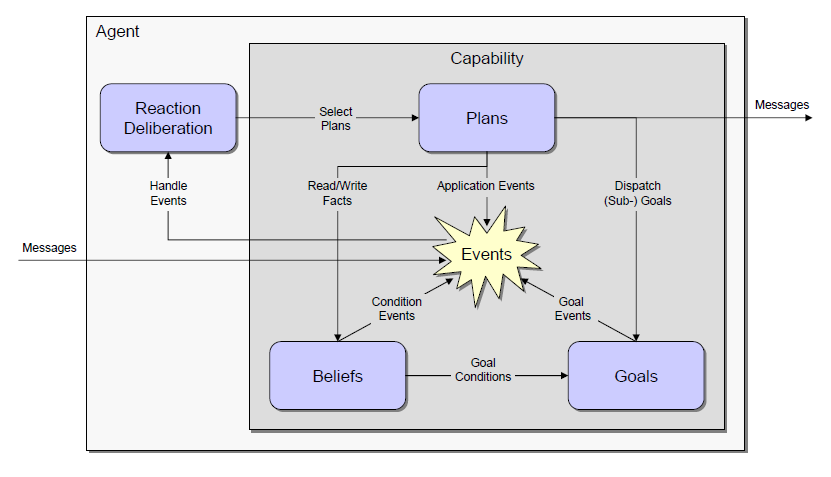
\includegraphics[width=300px]{images/Jadex_agent.png}
	\caption{Jadex abstract agent \cite{pokahr_jadex_2005}}
	\label{fig2}
\end{figure}
\autoref{fig2} depicts an abstract view on a Jadex agent. Every agent may receive messages which trigger internal events that can change his internal knowledge, plans or goals. Interactions with the outside like the environment or other agents happens through the sending of messages. % TODO @manuelmittler I removed the quote as I did not find it to be necessary here. Am I correct that modifications in the environment are also done through messages? -> what do you mean by "modifications in the environment"?
In more detail, beliefs are single facts stored as Java objects which represent the knowledge of an agent. % TODO @manuelmittler should I know, what a fact is? Because I honestly don't.. -> Didn't you attend some logic lectures?
They are stored as key-value pairs.
The advantage of storing information as facts is that the programmer has a central place for the knowledge and can query the agent's beliefs. % TODO @manuelmittler or do you mean that there is an advantage by storing them as Java Objects? -> yes
Monitoring of the beliefs is possible too.

The goals are momentary desires of an agent for which the agent engages into suitable actions until it considers the goal as being reached, unreachable, or not wanted any more.
Referring to \cite{ActiveComponentsGoals}, Jadex distinguishes between four generic goal types. 
A perform goal is directly related to the execution of actions.
Therefore, the goal is considered to be reached, when some actions have been executed, regardless of the outcome of these actions.
An achieve goal is a goal in the traditional sense, which defines a desired world state without specifying how to reach it.
Agents may try several different alternative plans, to achieve a goal of this type.
A query goal is similar to an achieve goal, but the desired state is not a state of the (outside) world, but in internal state of the agent, regarding the availability of some information the agent wants to know about.
For goals of type maintain an agents keep track of a desired state, and will continuously execute appropriate plans to re-establish this maintained state whenever needed.
In contrast to goals, events are (per default) dispatched to all interested plans but do not support any BDI-mechanism.
Therefore, the originator of an internal event is usually not interested in the effect the internal event may produce but only wants to inform some interested parties about some occurrence.
Plans represent the behavioural elements of an agent and are composed of a head and a body part.
The plan head specification is similar to other BDI systems and mainly specifies the circumstances under which a plan may be selected, e.g. by stating events or goals handled by the plan and preconditions for the execution of the plan.
Additionally, in the plan head a context condition can be stated that must be true for the plan to continue executing.
The plan body provides a predefined course of action, given in a procedural language.
This course of action is to be executed by the agent, when the plan is selected for execution, and may contain actions provided by the system API, such as sending messages, manipulating beliefs, or creating sub-goals (cf. \cite{braubach_jadex_2004})

Jadex is not based on a new agent programming language.
Instead, a hybrid approach is chosen, distinguishing explicitly between the language used for static agent type specification and the language for defining the dynamic agent behaviour.
An agent in Jadex consists of two components: An \emph{agent definition file} (short: ADF) for the specification of beliefs, goals, and plans as well as their initial values and on the other hand procedural plan code.
\begin{figure}
	\centering
	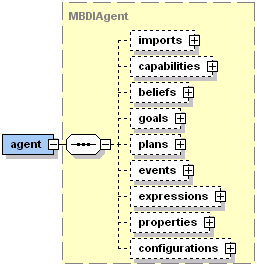
\includegraphics[height=200px]{images/jadexagentadf.png}
  \caption{Jadex top level ADF elements \cite{ActiveComponents}}
	\label{fig3}
\end{figure}
The procedural part of plans (the plan bodies) are realized in an ordinary programming language (Java) and have access to the BDI facilities of an agent through an application interface (API).
The plan body is a standard Java class that extends a predefined Jadex framework class and has at least to implement the abstract body() method which is invoked after plan instantiation.
\begin{lstlisting}
public class ServeCoffeePlanB1 extends Plan {
   // Plan attributes.

   public ServeCoffeePlanB1() {
       // Initialization code.
   }

   public void body() {
       // Plan code.
   }
}
\end{lstlisting}
The plan body is associated to a plan head in the ADF.
This means that in the plan head several properties of the plan can be specified, e.g. the circumstances under which it is activated and its importance in relation to other plans.
\begin{lstlisting}
<agent xmlns="http://jadex.sourceforge.net/jadex-bdi"
 xmlns:xsi="http://www.w3.org/2001/XMLSchema-instance"
 xsi:schemaLocation="http://jadex.sourceforge.net/jadex-bdi
                      http://jadex.sourceforge.net/jadex-bdi-2.0.xsd"
 name="CoffeeAgent">

 <plans>
   <plan name="serve">
     <body class="ServeCoffeePlanB1"/>
     <waitqueue>
       <messageevent ref="request_serving"/>
     </waitqueue>
   </plan>
 </plans>

 <events>
   <messageevent name="request_serving" direction="receive" type="fipa">
     <parameter name="performative" class="String" direction="fixed">
       <value>jadex.bridge.fipa.SFipa.REQUEST</value>
     </parameter>
   </messageevent>
 </events>

 <properties>
   <property name="debugging">false</property>
 </properties>

 <configurations>
   <configuration name="default">
     <plans>
       <initialplan ref="serve"/>
     </plans>
   </configuration>
 </configurations>
</agent>
\end{lstlisting}
There are two types of plans in Jadex.
A \emph{service plan} and a \emph{passive plan}.
The service plan, as the name indicates, is an instance of a plan which waits for service requests.
Therefore a service plan can set up its private event wait queue and receive events for later processing, even when it is working at the moment.
In contrast to that, a passive plan is only running when it has a task to achieve.
For this kind of plan the triggering event and goals must be specified must be specified in the agent definition file to let the agent know what kinds of events this plan can handle.
When an agent receives an event, the BDI reasoning engine builds up the so called applicable plan list which contains all plans that can handle the current event or goal.
The candidates are selected and instantiated for execution.

The execution model for Jadex looks like the following:
\begin{figure}
	\centering
	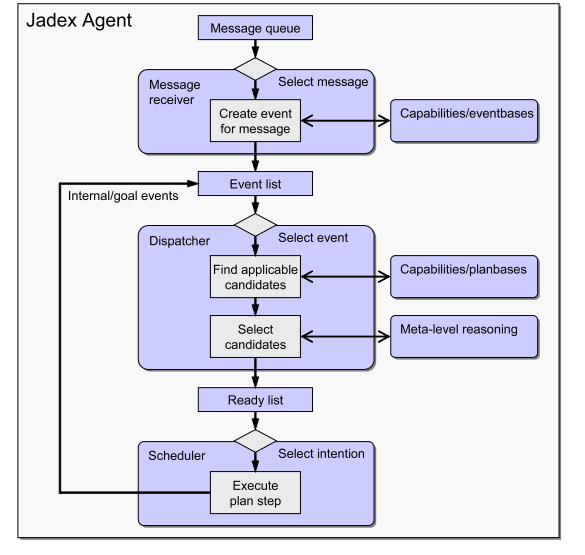
\includegraphics[width=300px]{images/Jadex_execution_model.png}
	\label{fig4}
	\caption{Jadex execution model \cite{pokahr_jadex_2005}}
\end{figure}
\newline
When an agent receives a message it is placed at a message queue.
In the next step the message has to be assigned to a capability, which can handle the message.
A suitable capability is found by matching the message against the event templates defined in the event base of each capability.
The best matching template is then used to create an appropriate event in the scope of the capability.
After that the created event is subsequently added to the agent's global event list.
The dispatcher is responsible for selecting applicable plans for the events from the event list.
After plans have been selected, they are placed in the ready list, waiting for execution.
The execution of plans is performed by a scheduler, which selects plans from the ready list.\cite{pokahr_jadex_2005}

All in all Jadex is a powerful framework that supports easy agent construction with XML-based agent description and procedural plans in Java.
Additionally, it offers tool support for development debugging.
It comes for example with a BDI-Viewer that allows observing and modifying the internal state of an agent and a logger agent that collects log-outputs of any agent.
Judging from this knowledge, Jadex seems suitable for the purpose of competing in the multi-agent programming contest.
